% THIS TEMPLATE IS A WORK IN PROGRESS
% Adapted from an original template by faculty at Reykjavik University, Iceland

\documentclass{scrartcl}

% Adapted from an original template by Hlyni Arnórssyni, Reykjavik University, Iceland
%
% ------------------------------ SETTINGS
\usepackage{geometry}

\geometry{
	paper=a4paper, % Paper size
	top=2.5cm, % Top margin
	bottom=2.5cm, % Bottom margin
	left=2.5cm, % Left margin
	right=2.4cm, % Right margin
	headheight=0.75cm, % Header height
	footskip=1.5cm, % Space from the bottom margin to the baseline of the footer
	headsep=0.75cm, % Space from the top margin to the baseline of the header
	%showframe, % Uncomment to show how the type block is set on the page
}

\usepackage{blindtext}
%-------------------------------- Character encoding ----------------------------
\usepackage[T1]{fontenc}
\usepackage[utf8]{inputenc}

%----------------------------- Mathematics packages from AMS ---------------

\usepackage{amsmath, amsfonts, amsthm, amssymb}
\usepackage{braket, nicefrac}

% ----------- International System of Units
\usepackage{siunitx}

%------------------------------ Lists / numbers -------------------------
\usepackage{enumitem, multicol}

%------------------------------- Figure insertions --------------
\usepackage{graphicx, float}  % Use option [H] to force the placement of a figure
\usepackage{keystroke}
\usepackage{pgfplots}\usepgfplotslibrary{units}\pgfplotsset{compat=1.16}




%%%%%%%%%%%%%%%%%%%%%%%%%% Hyperlink References %%%%%%%%%%%%%%%%%%%%%%%%%%%
\usepackage{hyperref}

%--------------------% Storage Path for images %-----------------%
\graphicspath{{graphics/}{Graphics/}{./}}
\usepackage{graphicx,epsfig}
\usepackage{listings}
\usepackage{subcaption}
\hypersetup{
   colorlinks   = true,                               %Colours links instead of ugly boxes
   urlcolor     = blue,                               %Colour for external hyper links
   linkcolor    = blue,                               %Colour of internal links
   citecolor    = red,                                %Colour of citations
   setpagesize  = false,
   linktocpage  = true,
}
\graphicspath{ {fig/} }



\renewenvironment{abstract}{
    \centering
    \textbf{Abstract}
    \vspace{0.5cm}
    \par
    \begin{minipage}{0.7\linewidth}}{\end{minipage}
    \noindent\ignorespaces
}
% ------------------------------------------------------------------------------------------------------------------------

\begin{document}
%Title of the report, name of coworkers and dates (of experiment and of report).
\begin{titlepage}
	\centering
	
\includegraphics[width=0.6\textwidth]{GW_logo.eps}\par
	\vspace{2cm}
	%%%% COMMENT OUT irrelevant lines below: Data Science OR Computer Science OR none
	{\scshape\LARGE Data Science Program \par}
	\vspace{1cm}
	{\scshape\Large Capstone Report - Spring 2024\par}
	%{\large \today\par}
	\vspace{1.5cm}
	%%%% PROJECT TITLE
	{\huge\bfseries GRAG - Open Sourced Python Package Implementation of Retrieval-Augmented Generation\par}
	\vspace{2cm}
	%%%% AUTHOR(S)
	{\Large\itshape Arjun Bingly,\\ Sanchit Vijay,\\ Erika Pham,\\Kunal Inglunkar}\par
	\vspace{1.5cm}
	supervised by\par
	%%%% SUPERVISOR(S)
	Amir Jafari

\newpage
	\vfill
	\begin{abstract}
	    This report introduces GRAG (Good RAG), an open-sourced Python package providing an end-to-end implementation of Retrieval-Augmented Generation (RAG).
	    The package provides easy integration with various LLMs locally, and support for vector databases such as Chroma and DeepLake. It also provides a simple GUI implementation. This report details GRAG and its features.
	    Future work includes enhancement of the PDF parsing features, possible integration for other document types, as well as testing GRAG performance on graphs versus a traditional vector database and producing an evaluation suite.
	    Our documentation can be accessed at \url{https://g-rag.org/} and Git repo at \url{https://github.com/arjbingly/grag}.
	\vfill
    \end{abstract}
    \end{titlepage}
% Bottom of the page


\tableofcontents
\newpage
% ------------------------------------------------------------------------------------------------------------------------
\section{Introduction}

Figure 1 shows a basic Retrieval-Augmented Generation (RAG) pipeline. As the name implies, the process is two-part: retrieval and generation.
The input query and documents are first preprocessed into vectors through the embedding process.
The pipeline then retrieves data relevant to the query, performing a similarity search in the vector database. Once the retrieval process is complete, RAG utilizes an LLM to understand and preserve context. Then, RAG system integrates the retrieved information with the original query to provide a richer context for the generation phase.
In the generation step, the augmented query is processed by a large-language model (LLM), which synthesizes the information into a coherent and contextually appropriate response. The final output is then post-processed, if necessary, to ensure it meets the required specifications, such as correctness, coherence, and relevance.

\begin{figure}[H]
	\begin{center}
		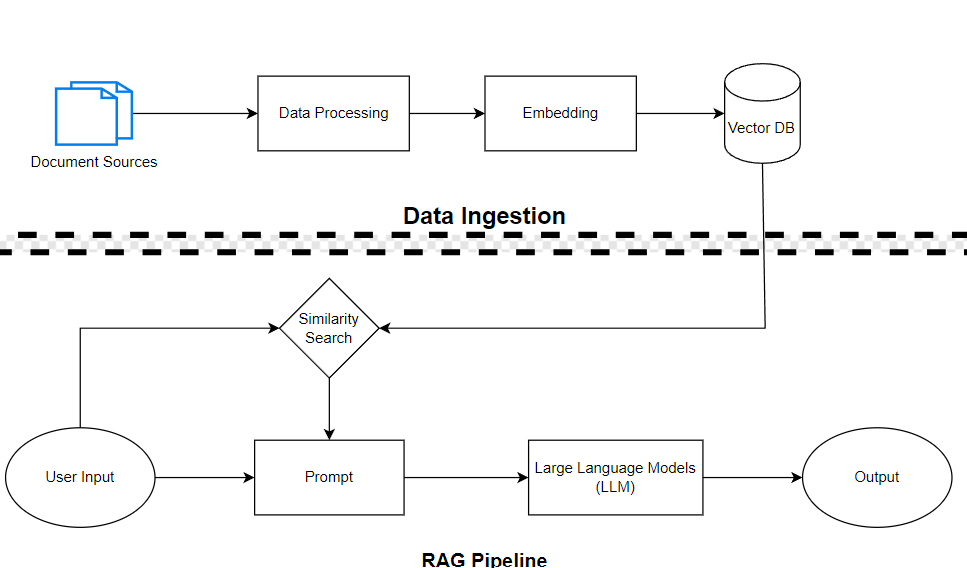
\includegraphics[scale=0.7]{capstone_report/fig/basic_RAG_pipeline.png}
	\end{center}
	\caption{Basic Retrieval-Augmented Generation (RAG) Pipeline}
	\label{fig:ascent}
\end{figure}

RAG provides several advantages and solutions to LLMs caveats:
\begin{itemize}
	\item Empowering LLM solutions with real-time data access:

	LLMs are typically trained on vast datasets that may quickly become outdated as new information emerges. RAG technology addresses this limitation by allowing LLMs to access and incorporate real-time data into their responses. Through the retrieval component, RAG systems can query up-to-date databases or the internet to find the most current information, ensuring that the generated output reflects the latest developments.
	\item Preserving data privacy:

	RAG can retrieve information from a controlled, secure dataset or environment rather than relying on direct access to private data. By designing the retrieval component to operate within privacy-preserving parameters, RAG can ensure that the LLM will not directly access or expose sensitive data.
	\item Mitigating LLM hallucinations:

	"Hallucination" in the context of LLMs refers to the generation of plausible but inaccurate or entirely fabricated information. This is a known challenge with LLMs, where the model might confidently produce incorrect data or statements.(cite) RAG helps mitigate this issue by grounding the LLM's responses in retrieved documents that are verified or deemed reliable. By leveraging external sources of information, RAG reduces the model's reliance on potentially flawed internal representations and biases, leading to more accurate outputs.
\end{itemize}
\newline
RAG has become very popular since its introduction in Lewis et al. 2020 \cite{lewis2021retrievalaugmented}, with its most-known implementation, ChatGPT (powered by GPT-4), creating a sizeable and long-term impact in all industries and academic institutions.
Its versatility in several fields has fueled interest in research and development to develop more RAG implementations. Our package, GRAG (Good RAG), aims to add to the RAG literature.

% ------------------------------------------------------------------------------------------------------------------------
\section{Problem Statement}

While RAG APIs such as OpenAI are very powerful, they usually have usage limits, which is a barrier for extensive commercial use.
Dependence on APIs could limit customization and integration to existing software, which is not ideal for institutions or individuals who have specific needs for their application.
Furthermore, sensitive data being stored on external servers, on top of data usage policy dependent on API providers; raise concerns of data privacy.
\newline
\newline
GRAG aims to provide a customizable, easy-to-use, end-to-end, open-sourced solution that resolves cost and data privacy issues. The package could be implemented locally, allowing for control over data storage and maximizing personalization.

% ------------------------------------------------------------------------------------------------------------------------

% ------------------------------------------------------------------------------------------------------------------------
\section{Features}

\subsection {PDF Parser}

Parsing PDF documents presents a significant challenge due to their complex structure. PDFs often contain unstructured data, which lacks a predefined organization, making accurate recognition and processing arduous. A notable difficulty arises when handling tables, as PDFs do not inherently understand table columns, complicating the task of recognizing table layouts. This complexity is particularly evident in documents like tax forms, which feature intricate nested table structures. Additionally, scanned PDFs require Optical Character Recognition (OCR) tools to convert images back into text, introducing another layer of complexity.
\newline
\newline
Initially, we tried only using \textit{unstructured.io}\cite{unstrio} and \textit{pdfplumber}\cite{pdfplumber}, respectively. Neither libraries could consistently parse all PDF files with high accuracy.
The current strategy is to primarily use the \textit{unstructured.io} library for partitioning and parsing.
For documents containing more complex table structures, such as nested tables or tax forms, \textit{pdfplumber} and \textit{pytesseract}\cite{pytesseract} are deployed.
The table structures on the documents are detected, then cropped out before the contained text is extracted from the tables.
\newline
\newpage
Below is an example of parsing a tax form, with a complex layout. We see that the output is fairly accurate in this case. The parsing tool is able to identify the layout and extract the information well.
\newline
\newline
\begin{figure}[h!]
    \centering
    \begin{subfigure}[b]{\textwidth}
        \includegraphics[width=\textwidth]{capstone_report/fig/og_form.png}
        \caption{Original Text}
        \label{fig:image1}
    \end{subfigure}

    \begin{subfigure}[b]{\textwidth}
        \includegraphics[width=\textwidth]{capstone_report/fig/og_form_output.png}
        \caption{Parsed Text}
        \label{fig:image2}
    \end{subfigure}
    \caption{Tax Form Parsing Example}
    \label{fig:images}
\end{figure}

\newline
\newline

This result is not consistent across all types of PDFs, however. Figure 6 (Appendix) is an example of how the tool extracts and parses a two-column paper. The layout is not accurate, and the text position is not in the right place. More experimentation is needed for a robust, consistent parsing tool for PDFs.


\subsection{Vector Stores}

Vector store or vector database is a type of database that stores data in high-dimensional vectors. This is a crucial component of RAG, storing embeddings for both retrieval and generation processes.
Currently, GRAG supports Chroma\cite{chroma} and DeepLake\cite{deeplake}. By default, our embedding model is instructor-xl, but any HuggingFace embeddings can be used.

\subsection{LLMs}
As explained above, cost and data privacy concerns mean we could not use OpenAI APIs. To run models locally, \textit{llama.cpp} is the best implementation as it uses a low-level language, with extensive backend support, such as CUDA.
Currently, GRAG provides two options to run LLMs locally:
\newline
\newline
1. Run LLMs using HuggingFace\cite{huggingface}:
\newline
This is the easiest way to get started, but does not offer as much flexibility. If using a config file (\textit{config.ini}), simply need to change the \textit{model\_name} to the HuggingFace repo id.
If the models are gated, user would need to provide an authentication token.
\newline
\newline
2. Run LLMs using llama.cpp \cite{langchain2023llamacpp}:
\newline
\textit{Llama.cpp} offers great flexibility, but its repository is not user-friendly. To streamline the process, we have a script/cookbook for ease of implementation.
\newline
\newline
GRAG has been tested with Llama2 7b \& 13b, Mixtral 8x7b, Gemma 13b, but could support any model from HuggingFace.
\newpage
\subsection{Multi-vector Retriever}

We built a retriever, which employs a Langchain tool called \textit{multi-vector retriever}.
Instead of representing each document as one vector, one document is represented by multiple vectors, with each vector being a different aspect of the text.
For example, the tool could split and then embed smaller chunks of a document, which would help embeddings to better carry semantic context.
Our retriever is used to retrieve multiple chunks and return the most similar chunks from a vectorDB.

\subsection{RAG Features}

\subsubsection{RAG Document Chains}

Document chains are used in Retrieval-Augmented Generation (RAG) to effectively utilize retrieved documents. These chains serve various purposes, including efficient document processing, task decomposition, and improved accuracy.
\newline
\newline

\begin{figure}[H]
    \centering
    \includegraphics[width=0.8\textwidth]{capstone_report/fig/stuff_chain_langchain.jpg}
    \caption{Illustration of Stuff Chain \href{https://readmedium.com/en/https:/ogre51.medium.com/types-of-chains-in-langchain-823c8878c2e9}{(LangChain)}}

\end{figure}
\newline
\textbf{Stuff Chain}
\newline
\newline
This is the simplest form of document chain. It involves putting all relevant data into the prompt. Given \(n\) documents, it concatenates the documents with a separator, usually \verb|\n\n|.
The advantage of this method is \textit{it only requires one call to the LLM}, and the model has access to all the information at once.
\newline
\newline
However, most LLMs can only handle a certain amount of context. For large or multiple documents, stuffing may result in a prompt that exceeds the context limit.
Additionally, this method is only suitable for smaller amounts of data. When working with larger data, alternative approaches should be used.

\begin{figure}[H]
    \centering
    \includegraphics[width=0.8\textwidth]{capstone_report/fig/refine_chain_langchain.jpg}
    \caption{Illustration of the Refine Chain method \href{https://readmedium.com/en/https:/ogre51.medium.com/types-of-chains-in-langchain-823c8878c2e9}{(LangChain)}}
\end{figure}
\newline
\textbf{Refine Chain}
\newline
\newline
The Refine Documents Chain uses an iterative process to generate a response by analyzing each input document and updating its answer accordingly.
It passes all non-document inputs, the current document, and the latest intermediate answer to an LLM chain to obtain a new answer for each document.
\newline
\newline
This chain is ideal for tasks that involve analyzing more documents than can fit in the model’s context, as it only passes one document to the LLM at a time.
\newline
However, this also means it makes significantly more LLM calls than other chains, such as stuff chain. It may perform poorly for tasks that require cross-referencing between documents or detailed information from multiple documents.
\newline
\newline
There may also be dependencies on the order in which the documents are analyzed, thus it might be ideal to provide documents in order of similarity.


\subsubsection{Prompting}
\newline
\newline
In additional to model-specific prompting, GRAG provides cookbooks to implement custom generic and few-shot prompts. To use, user needs to download and quantize a model, and ingest their document(s) of choice. As an example, we have ingested the United States Constitution to demonstrate custom prompting. Figure 5 shows an example of a custom prompt output.

\begin{figure}[H]
    \centering
    \includegraphics[width=\textwidth]{capstone_report/fig/custom_prompt_cookbook.png}
    \caption{Custom Prompt Cookbook Example}
\end{figure}
\newpage
\noindent "Query: What is the first amendment?" shows the input question.
\newline
\newline
The generated text is: "The First Amendment protects citizens from government interference with their fundamental rights, including freedom of speech, religion, the press, assembly, and petition. It also prohibits the government from establishing a national religion or abridging the right to bear arms without proper justification. Additionally, it provides for due process of law and a speedy trial by an impartial jury in criminal cases."
\newline
\newline
The module output also shows three "Sources" of where the pipeline got the generated information from.

\subsubsection{Other Hyperparameters}
\begin{itemize}
    \item \textbf{Chunk Sizes} --- generally, the smallest chunk size you can get away with.
    \item \textbf{Similarity Score} --- e.g., cosine similarity, a measure used to determine how similar two documents or vectors are.
    \item \textbf{Embedding} --- a representation of text in a high-dimensional vector space, which allows for capturing the semantic meaning of words or phrases.
\end{itemize}

\subsection{GUI}
GRAG provides a RAG GUI cookbook that you can run using Streamlit. To run, you need to download and quantize the LLM models, and ingest the documents you would like to use. As an example, we loaded the United States Constitution as a demo."Temperature" toggle decides how "creative" the generated answer is, and "Top-k" toggle decides how many relevant chunks to retrieve.

\begin{figure}[H]
    \centering
    \includegraphics[width=0.8\textwidth]{capstone_report/fig/gui.png}
    \caption{U.S. Constitution GUI Demo}

\end{figure}
\newline


% ------------------------------------------------------------------------------------------------------------------------

\section{Challenges \& Future Work}

\subsection{Evaluation}
\newline
When evaluating a RAG pipeline, we assess the performance of both the retrieval and generation processes. For retrieval, we measure how relevant the retrieved information is using precision/recall metrics. For generation, we examine the quality of the generated answer based on the retrieved content.
\newline\newline
For generation evaluation, traditional metrics such as ROUGE and BLEU calculate performance based on number of n-gram overlaps between generated text and a reference text. They are particularly limited; they do not correlate well with human evaluation \cite{sai2020survey}. Recently, LLMs have been proposed as a solution for reference-free end-to-end evaluation of question-answer pipelines like RAG. These models can be employed to predict the likelihood of a generated answer being correct based on context understanding rather than reference texts.
\newline
\newline
Currently, the most promising framework is Ragas \cite{es2023ragas}. However, it requires \mbox{OpenAI} to assess the performance. This is rather problematic for our project, since we have limited resources.

\subsection{Document Parsing}
\newline
While we have made improvements in parsing PDF files, the results are not consistent for different PDF layouts. More experimentation is needed to produce a more robust and accurate result. We also plan to implement parsing for more file types, such as HTML.

\subsection{Graphs Implementation}
\newline
Traditionally, RAG implementations uses vector databases for its retrieval process. As RAG uses vector embeddings for its processes, vector database is the optimal choice for ease of retrieval and efficiency in similarity search.
However, since RAG simply outputs the closest vector by means of cosine similarity, it leaves room for error if the database does not contain relevant information to the input prompt. This makes RAG overly reliant on the quality of the data and the embedding process.
\newline
\newline
Graphs present a very promising possibility due to its complex relational network - in theory, this could solve vector DB's limitation and reliance on cosine similarity.
There is limited existing literature comparing the performance of vector versus graph structure in a RAG implementation. Our next step is to implement graph database for GRAG, and compare its performance to vector databases.
\newpage
% ------------------------------------------------------------------------------------------------------------------------

\bibliographystyle{IEEEtran}
\bibliography{references}



%------ To create Appendix with additional stuff -------%
\newpage
\appendix
\section{Appendix}
%Put data files, CAD drawings, additional sketches, etc.
\begin{figure}[h!]
    \centering
    \begin{subfigure}[b]{0.8\textwidth}
        \includegraphics[width=\textwidth]{capstone_report/fig/og_text.png}
        \caption{Original Text}
        \label{fig:image1}
    \end{subfigure}

    \begin{subfigure}[b]{0.8\textwidth}
        \includegraphics[width=\textwidth]{capstone_report/fig/og_text_output.png}
        \caption{Parsed Text}
        \label{fig:image2}
    \end{subfigure}
    \caption{Double-column Parsing Example}
    \label{fig:images}
\end{figure}
\end{document} 